%!TEX root = ../template.tex
%%%%%%%%%%%%%%%%%%%%%%%%%%%%%%%%%%%%%%%%%%%%%%%%%%%%%%%%%%%%%%%%%%%%
%% chapter4.tex
%% NOVA thesis document file
%%
%% Chapter with lots of dummy text
%%%%%%%%%%%%%%%%%%%%%%%%%%%%%%%%%%%%%%%%%%%%%%%%%%%%%%%%%%%%%%%%%%%%

\typeout{NT FILE chapter4.tex}%

\chapter{Proposed Work}
\label{cha:proposed_work}

This chapter aims to outline the approach that will be used to achieve the project objectives defined in Chapter \ref{cha:introduction}, while providing the prior work in the various areas relevant to this study.

\section{Requirements}
\label{sec:requirements}

This section describes the requirements and functionalities to be developed during this dissertation, categorized into the following areas: Interactive Map, \gls{3D} Model Interaction, Repository, and \gls{VR} environment.

Given the diverse requirements of this project, the primary focus will be on developing an immersive \gls{VE}, prioritizing \gls{3D} models and \gls{VR} for exploring glass artifacts within the tomb. The interactive map features will be included but may be implemented with less detail.

\subsection*{Interactive Map}
A map of the Troia archaeological site under study will be incorporated into the project to offer interactive functionalities.
\begin{itemize}
    \item \textbf{Map Zoom \& Navigation:} Users can pan, zoom, and explore different locations.
    \item \textbf{Perspective Switching:} Toggle between top-down and profile views for better spatial understanding.
    \item \textbf{Geospatial Data Integration:} Include \gls{GIS} layers combining excavation findings, and overlay a \textit{.tif} map illustration with some immersive interaction.
    \item \textbf{Layer Toggle:} Toggle visibility of layers, such as excavation campaigns or glass antiquities.
    \item \textbf{Parallel Objects:} Link parallel excavation findings/museums, possibly integrating them in the object pop-up on the map.
\end{itemize}

\subsection*{\gls{3D} Models \& Interaction}
A dedicated component will focus on the interaction with \gls{3D} models, which will later be integrated into a \gls{VR} environment.
\begin{itemize}
    \item \textbf{Artifact Interaction:} Allows users to virtually manipulate (rotate, zoom etc) the glass artefact models, as well as apply different textures.
    \item \textbf{Contextual Overlay:} Display descriptive metadata about the artefact, such as its origin, period, and historical usage.
    \item \textbf{Reconstructed Models:} Showcase how artefacts would look originally (having in consideration characteristics such as: colourless glass, archaeological drawings and symmetry). However, due to time constraints and the need to model the original artefacts, the reconstruction functionality may not be completed.
    \item \textbf{3D Models Integration:} The user can zoom the map to visualize the perspective of a specific \gls{3D} model.
    %select a position to visualize the perspective of their 3D model.
\end{itemize}

\subsection*{Repository}
The repository will consist of a spatial database designed to store and manage data from the mausoleum under study.
\begin{itemize}
    \item \textbf{Document Upload/Download:} Allow contributors to upload images, videos or excavation reports of the archaeological intervention.
    \item \textbf{Search and Filter Features:} Users can search and filter based on some fields, such as time period, shape, and provenance.
    \item \textbf{Digital Preservation:} The usage of open, and standard formats to ensure a long-term resource access.
\end{itemize}


\subsection*{\gls{VR} Environment}
\gls{VR} functionalities will provide an intuitive user experience, enabling interaction with the \gls{VE} through the use of \glspl{HMD}.
\begin{itemize}
    \item \textbf{Immersive Experience:} \gls{VR} allows users to immerse in a virtual tomb visit, enabling interaction with glass relics.
    \item \textbf{Device Accessibility:} Primarily user-friendly and enabling haptic interaction, while supporting \gls{VR} glasses as an emerging display option.
    \item \textbf{Localization \& Wayfinding:} 
    \begin{itemize}
        \item \textbf{\gls{POI}:} Use colors, text, visual markers, or direction arrows to emphasize and guide users to historically significant locations.
    \end{itemize}
   % \item \textbf{Multilingual Support:} Provide language options to ensure accessibility for an international audience.
\end{itemize}

\section{Development Technologies and Tools}
\label{sec:technologies}

The following section focuses on the technologies and tools that will be used in the implementation of this project. These include frontend, backend, database, and \gls{3D} development tools.

\subsection{Web Mapping Development}

\subsubsection{Frontend Technologies}
\label{sec:frontend}

JavaScript is a programming language mostly used to control interactive behavior in web
pages. To make a map interactive, most websites automatically send JavaScript code to the browser~\cite{ajayi2024utilizing}. In this project, this language will be used for client-side web development and to integrate frameworks that enhance map interactivity.

Leaflet\footnote{\url{https://leafletjs.com/}} is an open-source JavaScript library that facilitates the creation of mobile-friendly interactive maps. It offers a wide array of plugins that improve usability and simplify application development.
Leaflet will be employed in this thesis to integrate interactive map features and create an intuitive user interface.

Other alternatives for web development frameworks used for map rendering and interaction include OpenLayers\footnote{\url{https://openlayers.org/}}, which enables the integration of dynamic maps into web pages and can display map tiles, vector data, and markers loaded from any source.
Another powerful tool is the Google Maps API\footnote{\url{https://developers.google.com/maps}}, which allows developers to embed Google Maps functionalities directly into both web and mobile applications.
Additionally, Mapbox\footnote{\url{https://www.mapbox.com/}} and \gls{OSM}\footnote{\url{https://www.openstreetmap.org/}} provide online mapping solutions. While \gls{OSM} is open-source, offering greater flexibility and customization, and is maintained and updated by the community, Mapbox and Google Maps API have usage-based pricing plans.
For this dissertation, one of these technologies will be used to create an interactive map, complementing an existing illustration of the Troia site area, that includes the mausoleum under study. This will be supplemented with an open map, potentially sourced from \gls{OSM}\footnote{\url{https://www.openstreetmap.org/}}.

\subsubsection{Backend Technologies}
\label{sec:backend} 

The backend technology selected for this thesis is Node.js, an open-source, cross-platform JavaScript runtime environment. Node.js enables developers to create servers, web applications, command-line tools, and automation programs.

In this project, Node.js will be used to support the web server and to improve performance and scalability when handling repository data. Additionally, it will streamline the communication between the backend and the database repository.


\subsection{Unity Engine}
\label{sec:unity_description} 

Unity is a cross-platform engine that provides a robust environment for developing \gls{2D} and \gls{3D} applications. 
Its component-based architecture simplifies \gls{3D} development by allowing developers to define object behaviors through scripts in \glspl{VE}.
Despite not being open-source, Unity offers a community forum and repositories where developers can access resources, and adapt them for their projects.
Additionally, the Unity Learn\footnote{\url{https://learn.unity.com/}} platform provides free tutorials, simplifying the learning process.

Unity will be a fundamental technology for supporting the \gls{VR} development of this project. Its integration enables users an immersive experience by visualizing several \gls{3D} data types, including excavation and glass artefacts metadata. 
Additionally, C\# programming language within Unity facilitates the management of game objects and user interactions in the \gls{VE}.


\subsection{Database Repository}
\label{sec:repos}

There are several alternatives for storage management systems, but the options are more limited when it comes to geographical
database systems.

For this project, organizing the data in a relational database is more appropriate due to its flexibility and consistency.
The most common databases for such applications include PostGIS, extension for PostgreSQL, MySQL\footnote{\url{https://www.mysql.com/}} and Oracle.
All three databases databases support spatial data types, allowing to store and manage geographic objects, representing them with points, lines, or polygons, and performing geospatial queries.
Among these, PostGIS is widely used for spatial data storage, geometry processing, and efficient geospatial querying.
Oracle supports advanced spatial features and 3D features but has a commercial license. On the other hand, MySQL is open-source and more suitable for small-to-medium-scale projects.

PostgreSQL database was chosen for this thesis because of its high performance and flexibility in managing spatial data. All geographic data, artefacts metadata, and excavation details will be stored within this system.


\subsection{Photogrammetry Tools}
\label{sec:photogrammetry_tool} 

The software that will be used to process digital images and generate \gls{3D} object models is \textit{Agisoft Metashape}\footnote{\url{https://www.agisoft.com/}}.
This software performs photogrammetric processing of digital images to generate \gls{3D} spatial data, which can be applied in various fields such as \gls{GIS} applications, \gls{CH} documentation, visual effects production, and indirect measurements of objects of diverse scales. 
By stitching together photographs, \textit{Agisoft Metashape} captures the geometry, texture, and visual appearance of physical objects or environments.
Other alternatives for photogrammetry softwares are Pix4D\footnote{\url{https://www.pix4d.com/}}, RealityCapture\footnote{\url{https://www.capturingreality.com/}} and DroneDeploy\footnote{\url{https://www.dronedeploy.com/}}

There are some already built models of the artefacts provided by Troia archaeologists, there will be done a selection and evaluation of the greatest possibilities.


\section{System Architecture}
\label{sec:architecture}

This section includes an overview of the system architecture. The communication flow between the layers will be conducted by a REST \gls{API}.
REST \glspl{API} with Node.js connects components in microservices architectures\footnote{\url{https://www.ibm.com/think/topics/rest-apis}}.
This service was selected due to its flexibility and lightweight solution. 

\begin{figure}[h!]
\centering
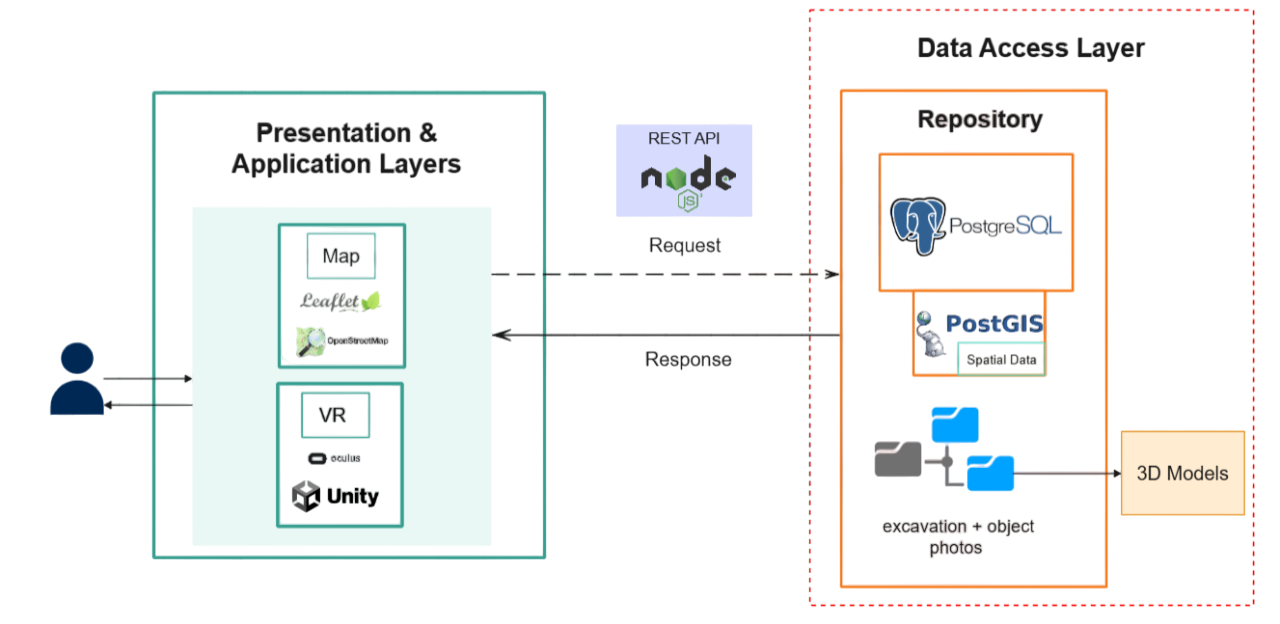
\includegraphics[width=1.0\linewidth]{system_architecture2}
\caption{System Architecture Overview}
\label{fig:architecture}
\end{figure}
\FloatBarrier

\section{Usability Tests}
\label{sec:usability_tests}

The Usability Tests will be conducted both remotely and presencially throughout the implementation process, specifically the \gls{HMD} interactions will be done in person.
Investigators from \gls{VICARTE} will participate in these tests with valuable feedback to improve the platform, while providing input on their archeology necessities. Their collaboration will contribute to a more useful, accurate, and user-friendly platform.

\section{Previous Work}
\label{sec:previous_work}

During the curricular internship, a platform was developed using React\footnote{\url{https://react.dev/}} and TailwindCSS for the web layer, with C\# and ASP.NET for the application layer, and MongoDB\footnote{\url{https://www.mongodb.com/}} for data storage. Communication between these three components was handled through direct requests to the web server, which forwarded \gls{CRUD} operations and interacted with the database.  
Additionally, the Database Systems and Cloud Computation Systems master's course provided hands-on experience in various storage methodologies and introduced different technologies and alternative solutions for data management.

This section explains the various experiments carried out during the preparation phase.

\subsection{Web \gls{GIS}}
\label{sec:gis_previous} 

To further develop expertise in \gls{GIS}, enrollment was made in the master's GeoWeb course taught by the thesis adviser, Armanda Rodrigues. During this course, was developed a Web \gls{3D} application designed to provide an interactive map for visualizing and analyzing demographic data, key infrastructure locations, and other notable European datasets. Although this project did not focus on archaeological data, it introduced and enriched the understanding of GIS concepts, map interaction, and geospatial analysis while exposing new technologies.

The application leveraged PostGIS, a PostgreSQL extension that supports spatial operations.
Additionally, frameworks like Leaflet were used for map rendering, visualization, and user interaction. For the base map, \gls{OSM} was integrated, offering a customizable and versatile visualization. This project serves as a preparatory stage for my thesis, specifically for the \gls{GIS} component, in which I will develop an interactive map of the Troia site.

\section{Data Structure Proposal}
\label{sec:data_strucutre}

A preliminary database structure has been proposed and analysed for artefacts storage management.  
It incorporates the key characteristics of each object to ensure structured organization and availability.

\begin{figure}[h!]
    \centering
    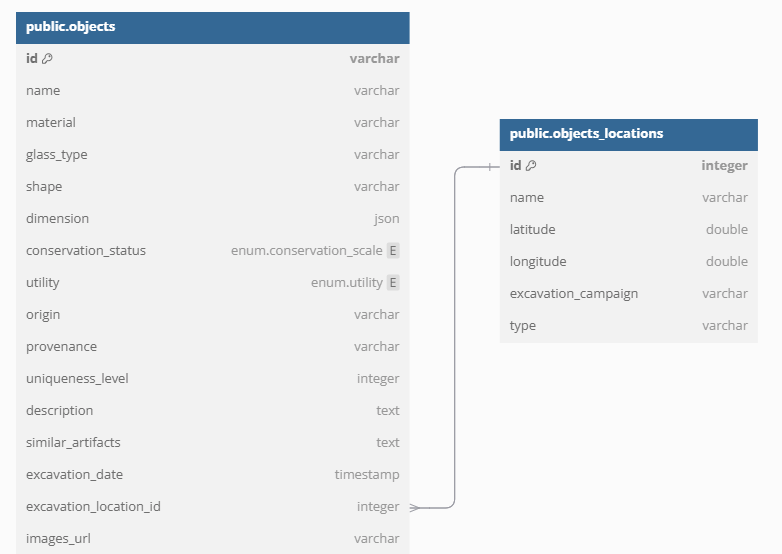
\includegraphics[width=0.7\textwidth]{data_structure}
    \caption{Proposed Data Structure for Managing Artifacts Data.}
    \label{fig:data_strucutre}
\end{figure}
\FloatBarrier

\subsection{Photogrammetry}
\label{sec:photogrammetry_previous} 

During the preparation, a photogrammetric experiment was conducted by the student using the \textit{Agisoft Metashape} environment. A total of 143 images were collected during the excavation campaign by the restoration department of NOVA for analysis. 
Based on these images, a \gls{3D} model was generated from the photogrammetric survey and subsequently imported into the \textit{Sketchfab} viewer for intuitive interaction.
Within the grave where the deceased was buried, three open triangular areas were identified, containing the precious artefacts of the defunct, as shown in Figure~\ref{fig:model3} below.

\begin{figure}[h!]
    \centering
    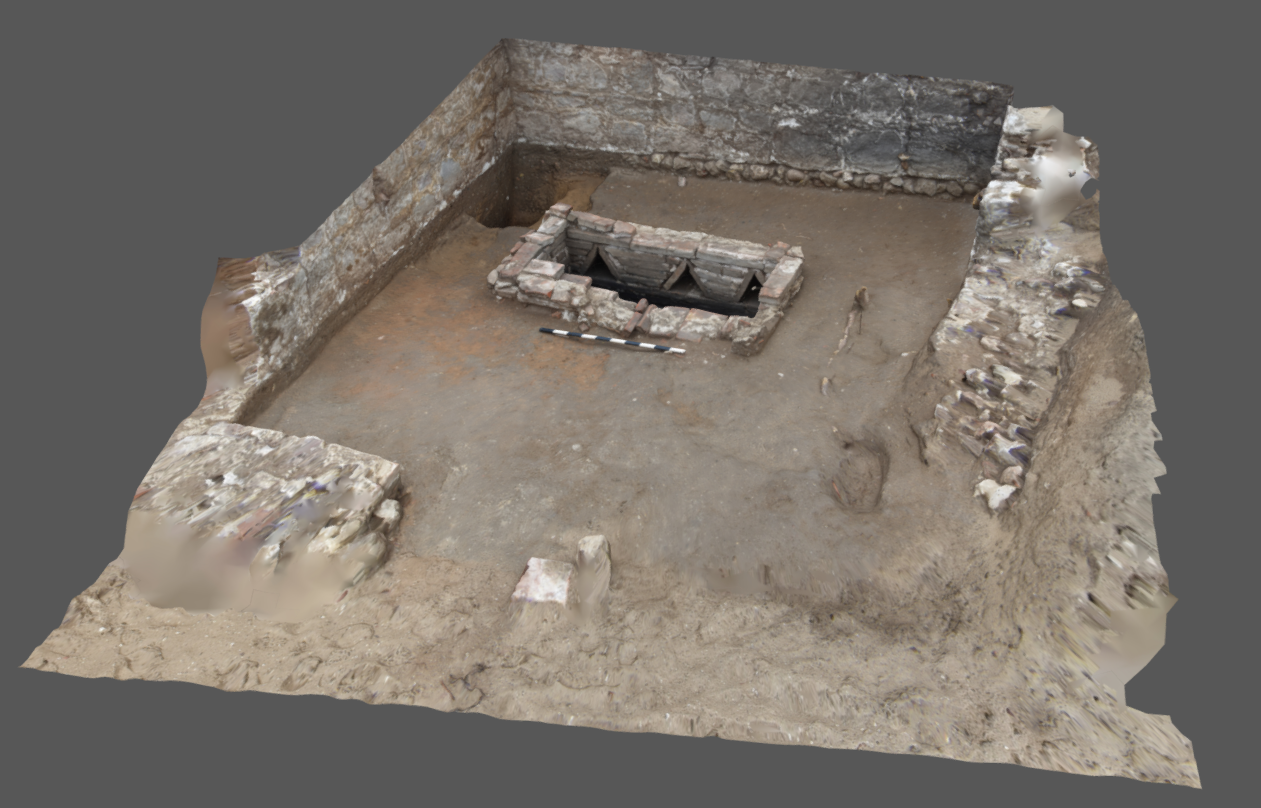
\includegraphics[width=0.7\textwidth]{model3}
    \caption{\gls{3D} Model Imported into Sketchfab for Visualization.}
    \label{fig:model3}
\end{figure}
\FloatBarrier

\subsection{Unity}
\label{sec:unity} 

To reproduce the visualization of the \gls{3D} models on the map, a simulation was created in Unity, as presented in Figure \ref{fig:overlay}. The goal was to overlay the map with the \gls{3D} excavation model.
To achieve this, the illustrated map was placed as the ground surface, with the excavation model positioned above it. The ultimate objective is to apply this approach to the artefacts found within the three triangular areas of the grave.

This experiment simulates an intended interactive and dynamic experience, allowing users to explore the map and objects through interactive layers while using an \gls{HMD}.

\begin{figure}[h!]
    \centering
    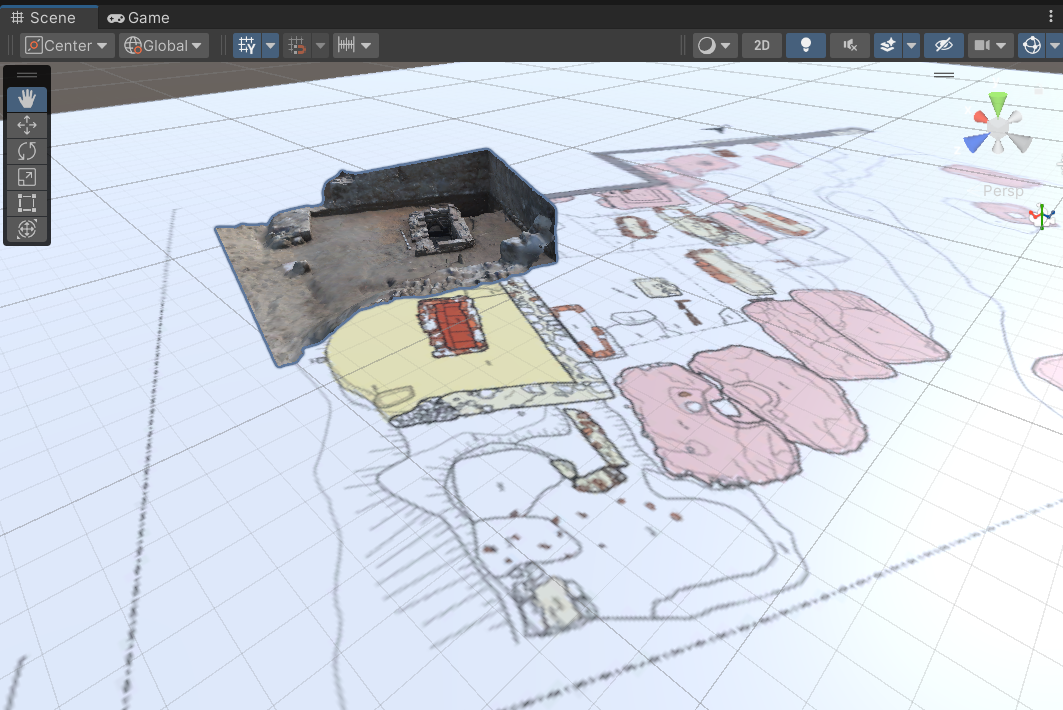
\includegraphics[width=0.7\textwidth]{overlay_test}
    \caption{Overlay \gls{3D} Excavation Model with a Map Representation.}
    \label{fig:overlay}
\end{figure}
\FloatBarrier


\section{Work Plan}
\label{cha:work_plan}

This section contains the planned progress, organized into distinct tasks, each with a description. Some tasks will be developed in parallel. 
Additionally, a Gantt chart is presented in Figure \ref{fig:gantt_chart} to illustrate the timeline for each task.

\begin{itemize}
    \item \textbf{Mockup Development}: This task focuses on developing a mockup that includes map visualization within a \gls{VE}, along with the associated functionalities and \gls{3D} models visualization.
    \item \textbf{\gls{VE} Development}: This phase involves creating an immersive environment where users can navigate, and select objects, followed by the implementation of interactive functionalities with \gls{3D} models of the artefacts. These interactions include applying filters, zooming, and scaling. Initially, the development will focus on a simulation with a single object.
    \item \textbf{\gls{GIS} Implementation}: This task comprises the creation of a map that allows user interaction with \gls{POI} represented by markers, integrating layers, and providing functionalities as outlined in Section \ref{sec:requirements}. Although the \gls{GIS} and \gls{VR} tools are developed in parallel, it may be possible to transfer from the map to the immersive environment through user interaction (e.g., clicking on a location on the map to display its \gls{3D} model), or the other way around.
    \item \textbf{Database Creation for Repository}: In this phase, a database will be established to store significant data, including artefact and excavation metadata. The structure will initially focus on a single object, as proposed in Section \ref{sec:data_strucutre}. The database will be continuously updated over several weeks to data loading and modifications.
    \item \textbf{System Evaluation \& Testing}: This task involves testing functionalities, usability, and performance, with participation from VICARTE investigators. Following the conclusion of the testing phase, the system evaluation process will begin with user questionnaires, leading to potential improvements based on the feedback received.  
    \item \textbf{Documentation}: The dissertation report will be developed during the whole process.
\end{itemize}

% \begin{figure}[h!]
%     \centering
%     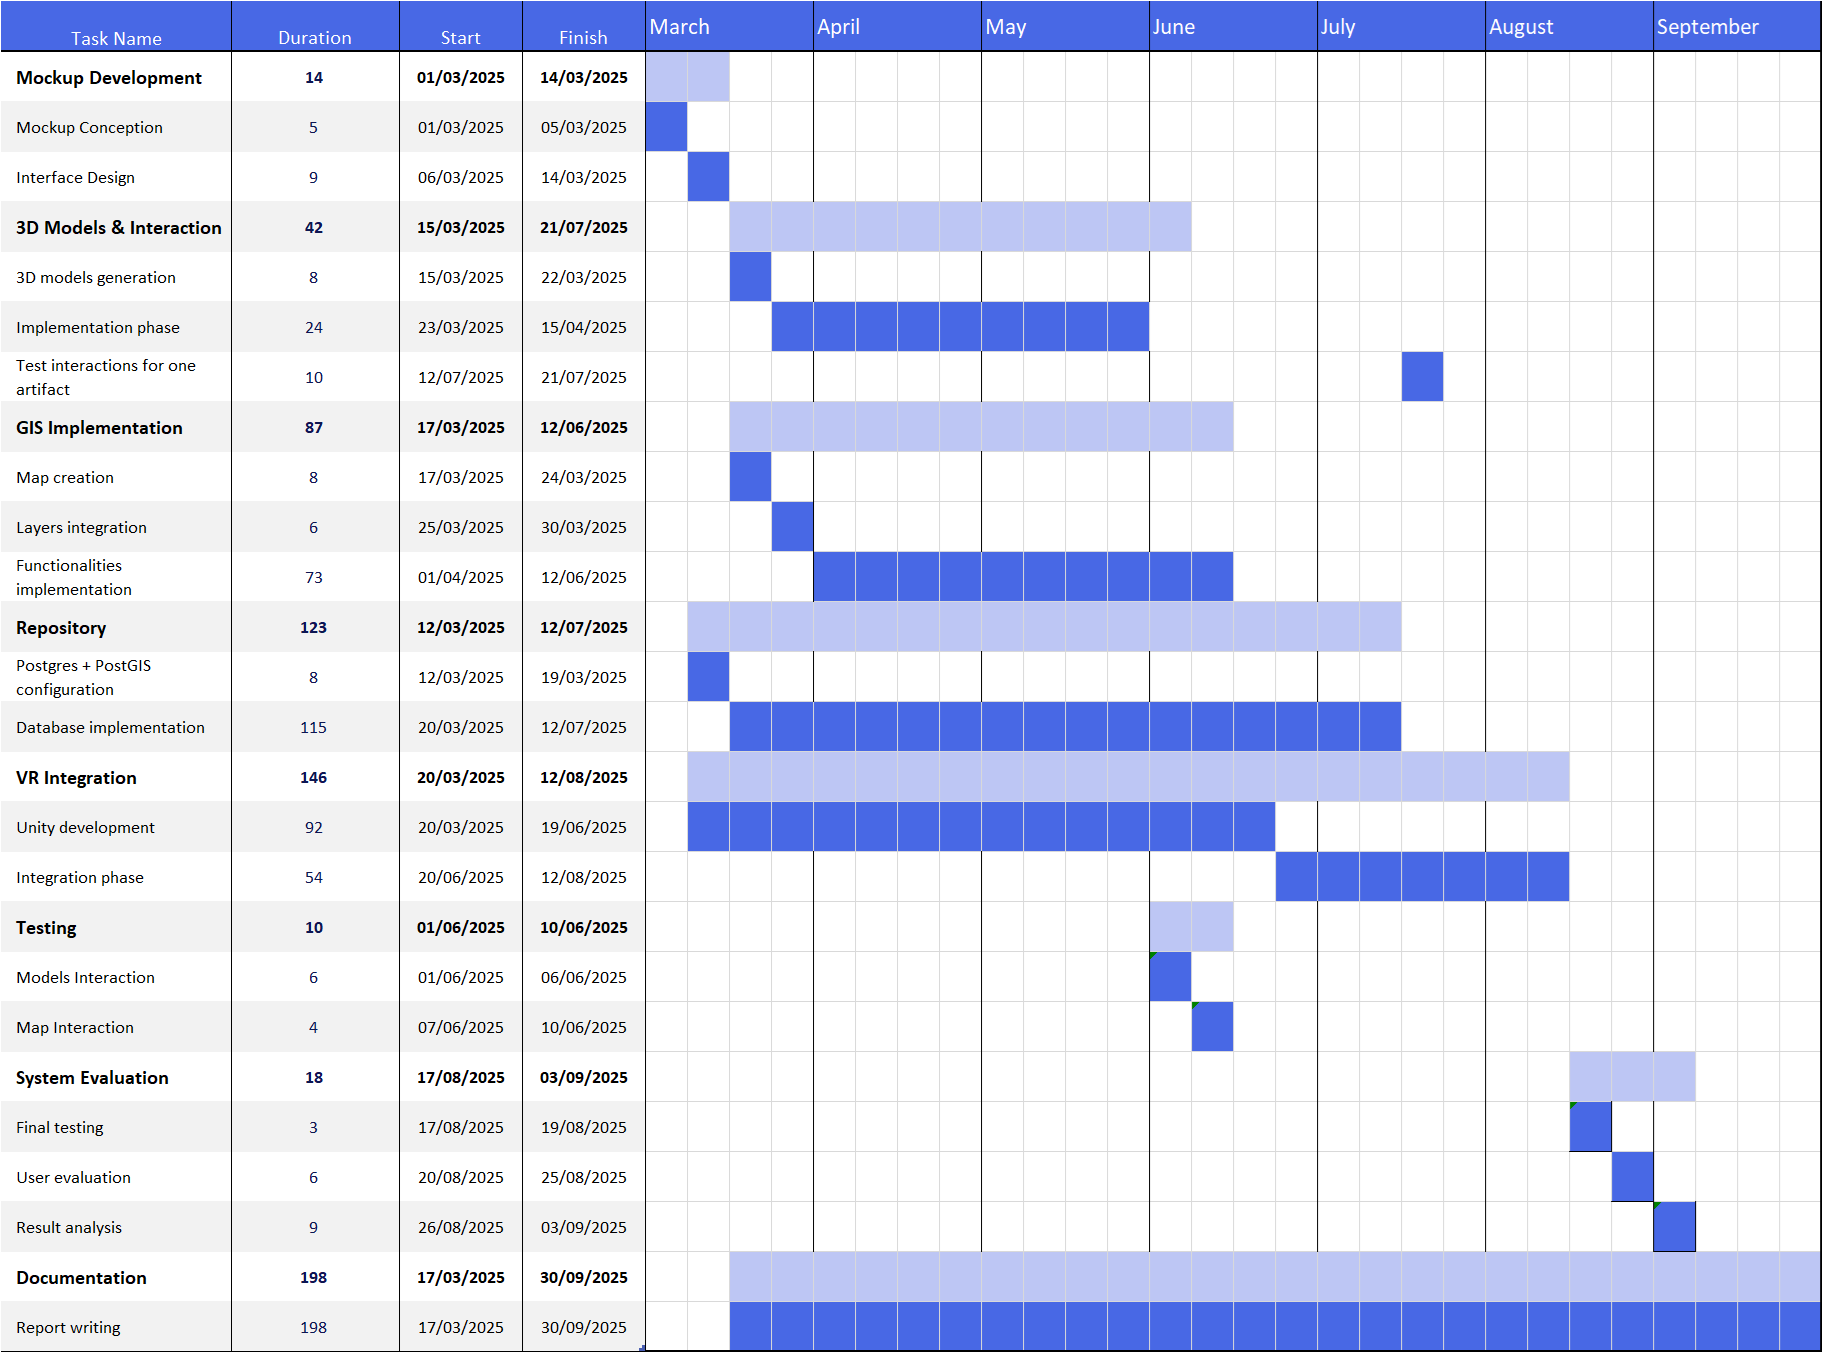
\includegraphics[width=1.0\linewidth]{Gantt_chart}
%     \caption{Gantt Chart Representation of the Work Plan.}
%     \label{fig:gantt_chart}
%   \end{figure}
%   \FloatBarrier


%   \begin{figure}[h!]
%     \centering
%     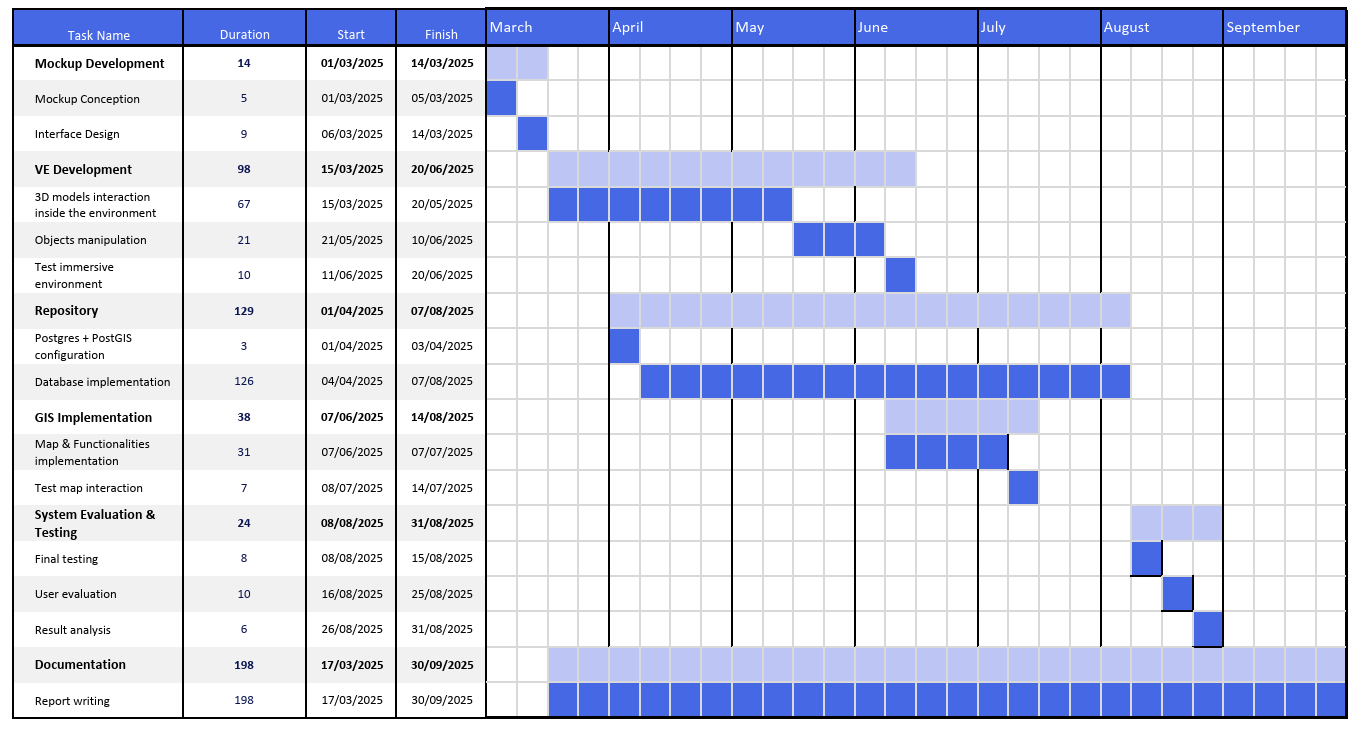
\includegraphics[width=1.0\linewidth]{gantt_chartt}
%     \caption{Gantt Chart Representation of the Work Plan.}
%     \label{fig:gantt_chart}
%   \end{figure}
%   \FloatBarrier

  \begin{figure}[h!]
    \centering
    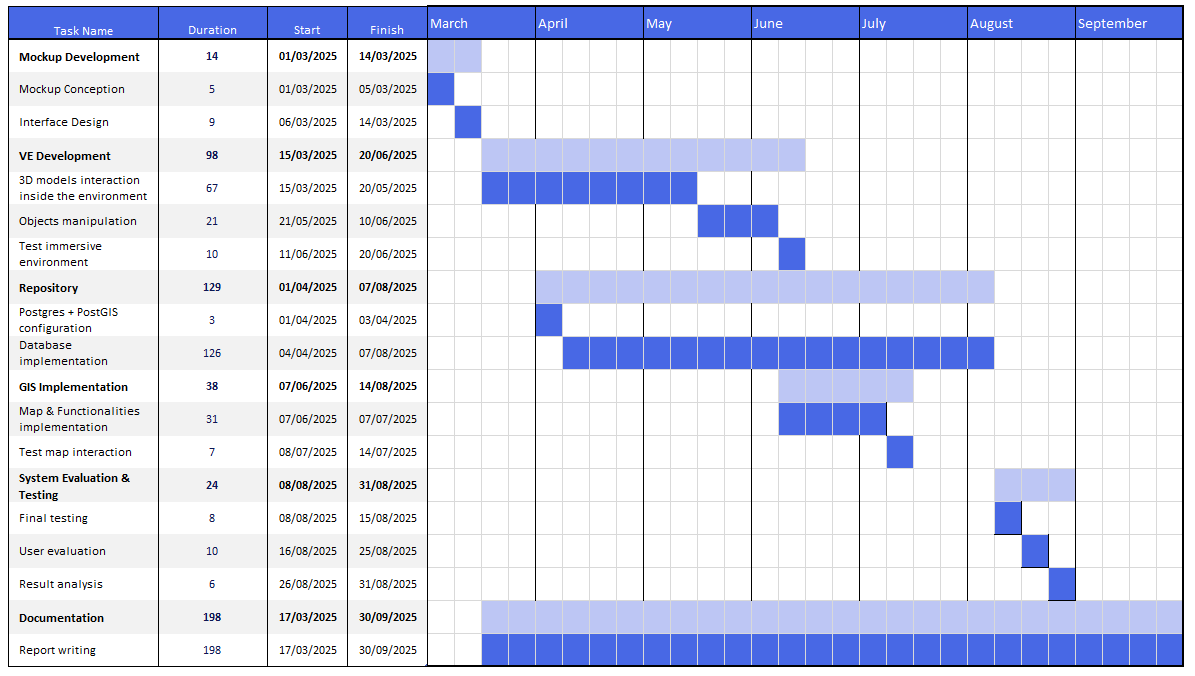
\includegraphics[width=1.0\linewidth]{gantt_chartt2}
    \caption{Gantt Chart Representation of the Work Plan.}
    \label{fig:gantt_chart}
  \end{figure}
  \FloatBarrier


